\documentclass[a4paper,11pt]{report}
\usepackage{polski}
\usepackage[utf8]{inputenc}
\usepackage{graphicx} % obrazki
\usepackage{fancyvrb} % spacje w verbatim
\usepackage[table]{xcolor}
\usepackage{geometry}
\usepackage{indentfirst}
\usepackage{arydshln}
\usepackage{tikz}
\usepackage{pgfplots}
\pgfplotsset{every tick label/.append style={font=\footnotesize}}
\title{Quicksort}
\author{Rafał Stępień Krzysztof Kotlarz}
\date{\today}
\begin{document}
\renewcommand{\tabcolsep}{10mm}
\newgeometry{tmargin=2cm,bmargin=2cm,lmargin=2cm,rmargin=2cm}

\begin{titlepage}
   \begin{center}
       \vspace*{9cm}
 
       \textbf{\huge{Quicksort - sortowanie szybkie}}
 
       \vspace{1.5cm}
 
       Rafał Stępień | Krzysztof Kotlarz \\
       \vspace{2cm}

 
       Wydział Biologii i Hodowli Zwierząt\\
       Uniwersytet Przyrodniczy we Wrocławiu\\
       Bioinformatyka\\
 
   \end{center}
\end{titlepage}
\newpage
\tableofcontents
\newpage
\chapter{Wprowadzenie}
\hspace{10pt} W przypadku rozważania efektywności algorytmu quicksort bierzemy pod uwagę przede wszystkim dwa przypadki: najlepszy i średni, więc to właśnie na nich skupimy swoje rozważania, można jednak wysnuć intuicje dotyczące przypadku najgorszego (który opiszemy pobieżnie).\\
\\
Wśród zalet algorytmu sortowania szybkiego możemy z pewnością wymienić działanie w miejscu, bardzo efektywny czas działania w średnim przypadku, oraz to, że działa nawet w środowiskach wykorzystujących pamięć wirtualną.
\section{Ogólny opis działania}
Algorytm jest oparty na technice "dziel i zwyciężaj", którą możemy podzielić na 3 kroki:
\begin{enumerate}
\item \textbf{Dziel} - Tablica $A[]$ jest dzielona na dwie części, takie, że każdy element tablicy pierwszej jest nie większy niż $A[q]$, a każdy element tablicy drugiej jest większy od $A[q]$. Możemy wywnioskować że bardzo ważnym krokiem będzie wybór elementu $A[q]$.
\item \textbf{Zwyciężaj} - Obydwie podtablice są sortowane rekurencyjnymi wywołaniami quicksort.
\item \textbf{Połącz} - Z racji tego, że sortowanie odbywa się w miejscu nie musimy łączyć tablic, ponieważ są one już automatycznie połączone.\\
\end{enumerate}
\subsubsection{Zalety}
\begin{itemize}
\item \textbf{Sortowanie w miejscu} - zaletą takiego działania jest to, że nie zużywamy dodatkowej pamięci, ponieważ operacje są wykonywane za każdym razem na tej samej liście, nie tworzymy nowej.
\item \textbf{Szybkość średniego przypadku} - jego oczekiwany czas działania wynosi $\theta(nlgn)$, a stałe ukryte pod znakiem $\theta$ są małe.
\item Działa dobrze w środowiskach wykorzystujących \textbf{pamięć wirtualną}
\end{itemize}
\section{Przypadki}
\subsubsection{Średni przypadek}
Złożoność obliczeniowa jak wyżej wspomnieliśmy wynosi w średnim przypadku $\theta(nlgn)$, co jest bardzo dobrym wynikiem, ze względu na powolny wzrost funkcji logarytmicznej (ryc. 1). \\
\\
\textit{ryc.1 - wykres dla funkcji $y=x$(czerwona), $y=x^2$(czarna - rosnąca szybciej), $y=log2(x)$(niebieska), $y=2^x$(zielona), $y=2log2(x)$(czarna - rosnąca wolniej), wygenerowany dzięki stronie: https://www.desmos.com/calculator}
\subsubsection{Najgorszy przypadek}
Istnieje też druga strona medalu i przypadek najgorszy $\theta(n^2)$

\subsubsection{Szukanie pivota}
Pivot możemy ustalać na różne sposoby. Najpopularniejszymi z nich jest wybór ostatniego elementu na liście, pierwszego elementu na liście, wybór elementu, który jest elementem środkowym spośród trzech (pierwszego, środkowego, ostatniego), lub możemy wybrać element losowo. Wszystkie te podejścia testujemy w naszym kodzie.
\subsubsection{Implementacja w pseudokodzie}
\begin{Verbatim}
Quicksort(A, p, r):
if p < r
	q = partition(A, p, r)
	quicksort(A, p, q-1)
	quicksort(A, q+1, r)
\end{Verbatim}


\section{Podział tablicy}
Dzięki funkcji def partition następuje podzielenie większych problemów na mniejsze. Wykorzystany zostanie pivot, czyli element który pozwoli wyznaczyć na dwa podproblmy. Elementy na lewo od pivot'a będą od niego mniejsze, zaś po jego prawej stronie, większe.


Procedurę zaczęto od wybrania wartości p, która ma być pivotem wg. jednej z 4 funkcji (wartość ze zbioru znajdująca się na: końcu, początku, w miejscu środkowym lub z losowego miejsca), względem której będzie dokonywany podział. Indeksem pivota zawsze zostaje miejsce będące ostatnią pozycją analizowanego przedziału.


Element $i$-ty to element obecnie poddawany analizie w ciele pętli. natomiast element $j$-ty jest to tzw. border 
w którego miejsce wstawiane będą elementy $i$-te. Ostatecznie border wyznacza miejsce w które trafić ma pivot po wyjściu z pętli oraz miejsce zawierające element posortowany, który znajduje się we właściwym miejscu. Pivot nie zostaje analizowany podczas iteracji


Procedurę zaczynamy zawsze od początku do końca wyznaczonego zbioru. Element $i$-ty zostaje zamieniony z $j$-tym w momencie, gdy i$<$p. Zbiór analizowany jest element po elemencie. Gdy następuje zamiana, element $j$ zostaje przesunięty $+1$. Komórki zaznaczone na szaro to elementy ulegające zamianie w danej iteracji.
\begin{table}[h!]
\Large
\centering
\begin{tabular}{|c|c|c|c|c|c|}
\hline
\cellcolor{black!25} &  &  &  &  & \\
\cellcolor{black!25}2 & 8 & 7 & 1 & 3 & 5 \\ \hdashline
i=j&  & &  &  & p\\ \hline
\end{tabular}

\end{table}

Element $i$-ty = 2 jest mniejszy od p$=$5. Zostaje on zamieniony z elementem $j$-tym. W tym przypadku następują zamiana w miejscu.

\begin{table}[h!]
\Large
\centering
\begin{tabular}{|c|c|c|c|c|c|}
\hline
 &  &  &  &  & \\
2 & 8 & 7 & 1 & 3 & 5 \\ \hdashline
 & i=j & &  &  & p\\ \hline
\end{tabular}

\end{table}

Po zamianie następuje przesunięcie elementu $j$-tego +1. Rozpoczęto analizę kolejnego $i$-tego elementu.

\begin{table}[h!]
\Large
\centering
\begin{tabular}{|c|c|c|c|c|c|}
\hline
 &  &  &  &  & \\
2 & 8 & 7 & 1 & 3 & 5 \\ \hdashline
 & j & i &  &  & p\\ \hline
\end{tabular}

\end{table}

\begin{table}[h!]
\Large
\centering
\begin{tabular}{|c|c|c|c|c|c|}
\hline
 & \cellcolor{black!25} &  & \cellcolor{black!25} &  & \\
2 & \cellcolor{black!25}8 & 7 & \cellcolor{black!25}1 & 3 & 5 \\ \hdashline
 & j &   & i &  & p\\ \hline
\end{tabular}

\end{table}

Elementy i$=$1 jest mniejszy od wartości $p=$5 zostaje zamieniony z elementem $j=$8


\begin{table}[h!]
\Large
\centering
\begin{tabular}{|c|c|c|c|c|c|}
\hline
 &  &\cellcolor{black!25}  &  & \cellcolor{black!25} & \\
2 & 1 & \cellcolor{black!25}7 & 8 & \cellcolor{black!25}3 & 5 \\ \hdashline
 &   & j  &   & i & p\\ \hline
\end{tabular}

\end{table}

Elementy i$=$3 jest mniejszy od wartości p$=$5 zostaje zamieniony z elementem $j=$7 

\begin{table}[h!]
\Large
\centering
\begin{tabular}{|c|c|c|c|c|c|}
\hline
 &  &  & \cellcolor{black!25} &  &\cellcolor{black!25} \\
2 & 1 & 3 & \cellcolor{black!25}8 & 7 &\cellcolor{black!25} 5 \\ \hdashline
 &   &   & j  &  & p\\ \hline
\end{tabular}

\end{table}

Pivot nie jest analizowany w pętli. Gdy pętla dobiegnie końca pivot $p$ zamieniany jest z elementem $j-$tym.


\begin{table}[h!]
\Large
\centering
\begin{tabular}{|c|c|c|c|c|c|}
\hline
\multicolumn{3}{|c|}{Lewa część tablicy} & Pivot & \multicolumn{2}{c|}{Prawa część tablicy} \\ \hline
2 & 1 & 3 & \textbf{5} & 7 & 8 \\ \hdashline
 &  &  &  &  &  \\ \hline
\end{tabular}

\end{table}

Duży problem został podzielony na dwa mniejsze; lewą oraz prawą część tablicy. W momencie pivot $p$ jest uważany za posortowany, który znajduje się we właściwym dla siebie miejscu. Następnie rekurencyjnie wywołujemy tą samą funkcje, jednak tym razem dotyczyć ona będzie jedynie jednego z podproblemów. Funkcja $partition$ analizować będzie teraz lewą część tablicy

\begin{table}[h!]
\Large
\centering
\begin{tabular}{|c|c|c|}
\hline
\multicolumn{3}{|c|}{Lewa część tablicy} \\ \hline
\cellcolor{black!25}2 & 1 & 3 \\ \hdashline
i=j &  & p \\ \hline
\end{tabular}

\end{table}

Procedura jest identyczna jak w przypadku pierwszego wykonania funkcji. Pozycja pivota $p$ znajduje się na ostatniej pozycji analizowanego zbioru. Iteracje rozpoczynamy od początku listy. 


Elementy $i=$2 jest mniejszy od wartości $p=$3 zostaje on zamieniony z elementem $j=$2. W tym przypadku następuje zamiana w miejscu.


\begin{table}[h!]
\Large
\centering
\begin{tabular}{|c|c|c|}
\hline
 & \cellcolor{black!25} &   \\
2 & \cellcolor{black!25}1 & 3 \\ \hdashline
 & i=j  & p \\ \hline
\end{tabular}

\end{table}

Po zamianie następuje przesunięcie elementu j-tego +1. Rozpoczęto analize kolejnego i-tego elementu. Elementy $i=$1 jest mniejszy od wartości $p=$3 zostaje on zamieniony z elementem $j=$1. W tym przypadku następuje zamiana w miejscu.


\begin{table}[h!]
\Large
\centering
\begin{tabular}{|c|c|c|}
\hline
 &  & \cellcolor{black!25}  \\
2 & 1 & \cellcolor{black!25}3 \\ \hdashline
 &   & j=p \\ \hline
\end{tabular}

\end{table}

Pivot nie jest analizowany w pętli. Gdy pętla dobiegnie końca pivot $p$ zamieniany jest z elementem $j$-tym.

\begin{table}[h!]
\Large
\centering
\begin{tabular}{|c|c|c|}
\hline
\multicolumn{2}{|c|}{Lewa część tablicy} & Pivot \\ \hline
2 & 1 & \textbf{3}\\ \hdashline
 &  &  \\ \hline
\end{tabular}
\end{table}

Pivot $p$ znajduje się we właściwym dla siebie miejscu. 
Następuje analiza kolejnego podproblemu. Zbiór składa się z lewej części tablicy zawierającej 2 elementy, oraz prawej części tablicy zawierającej 0 elementów.

\begin{table}[h!]
\Large
\centering
\begin{tabular}{|c|c|}
\hline
\multicolumn{2}{|c|}{Lewa część} \\ \hline
\cellcolor{black!25}2 & 1 \\ \hdashline
i=j & p \\ \hline
\end{tabular}

\end{table}


\begin{table}[h!]
\Large
\centering
\begin{tabular}{|c|c|}
\hline
\cellcolor{black!25} &  \cellcolor{black!25}\\ 
\cellcolor{black!25}2 & \cellcolor{black!25}1 \\ \hdashline
j & p \\ \hline
\end{tabular}

\end{table}

Pozycja pivota $p$ znajduje się na ostatniej pozycji analizowanego zbioru. Iteracje rozpoczynamy od początku listy. 


Element $i=$2 nie zostaje przeniesiony. Pivot $p$ nie jest analizowany, zamieniany jest z elementem $j$-tym.

\begin{table}[h!]
\Large
\centering
\begin{tabular}{|c|c|}
\hline
 Lewa część & Pivot \\ \hline
1 &  \textbf{2}\\ \hdashline
 &  \\ \hline
\end{tabular}
\end{table}


Pivot $p$ znajduje się we właściwym dla siebie miejscu.

\begin{table}[h!]
\Large
\centering
\begin{tabular}{|c|}
\hline
Lewa \\ \hline
\textbf{1} \\ \hdashline
 \\ \hline
\end{tabular}

\end{table}

Ze względu na warunek rekurencji $start < stop$ część jednoelementowa nie podlega analizie. Element znajduje się we właściwej dla siebie pozycji.

\begin{table}[h!]
\Large
\centering
\begin{tabular}{|c|c|c|c|c|c|}
\hline
\multicolumn{3}{|c|}{Lewa część tablicy} & Pivot & \multicolumn{2}{c|}{Prawa część tablicy} \\ \hline
2 & 1 & 3 & \textbf{5} & 7 & 8 \\ \hdashline
 &  &  &  &  &  \\ \hline
\end{tabular}

\end{table}

Kolejne wywołanie rekurencyjne będzie analizowało prawą część tablicy.


\begin{table}[h!]
\Large
\centering
\begin{tabular}{|c|c|}
\hline
\multicolumn{2}{|c|}{Prawa część} \\ \hline
\cellcolor{black!25}7 & 8 \\ \hdashline
i=j & p \\ \hline
\end{tabular}

\end{table}

Elementy $i=$7 jest mniejszy od wartości $p=$8 zostaje on zamieniony z elementem $j=$7. Następuje zamiana w miejscu.


\begin{table}[h!]
\Large
\centering
\begin{tabular}{|c|c|}
\hline
 &  \cellcolor{black!25}\\ 
7 & \cellcolor{black!25}8 \\ \hdashline
 & j=p \\ \hline
\end{tabular}

\end{table}
Po zamianie następuje przesunięcie elementu $j$-tego +1. Pivot $p$ zamieniany jest z elementem $j$-tym. Następuje zamiana w miejscu

\begin{table}[h!]
\Large
\centering
\begin{tabular}{|c|c|}
\hline
 Lewa część & Pivot \\ \hline
7 &  \textbf{8}\\ \hdashline
 &  \\ \hline
\end{tabular}

\end{table}

Pivot $p$ znajduje się we właściwym dla siebie miejscu. 

\begin{table}[h!]
\Large
\centering
\begin{tabular}{|c|}
\hline
Lewa \\ \hline
\textbf{7} \\ \hdashline
 \\ \hline
\end{tabular}

\end{table}

Pivot $p$ znajduje się we właściwym dla siebie miejscu. Ze względu na warunek rekurencji część jednoelementowa nie podlega analizie. Element znajduje się we właściwej dla sienie pozycji.


Po "sprasowaniu" wszystkich elementów \textbf{pogrubionych} otrzymamy posortowaną listę.


\section{Implementacja w Python}
\subsection{Quicksort}
\begin{Verbatim}
def quick_sort(lst, start, stop, fun):
    if start < stop:
        border = fun(lst, start, stop)
        quick_sort(lst, start, border - 1, fun)
        quick_sort(lst, border + 1, stop, fun)
\end{Verbatim}
\subsection{Partition}
\begin{Verbatim}
def partition(lst, start, stop):
    pivot_index = stop
    pivot_value = lst[pivot_index]
    for i in range(start, stop):
        if lst[i] < pivot_value:
            lst[i], lst[start] = lst[start], lst[i]
            start += 1
    lst[stop], lst[start] = lst[start], lst[stop]
    return start
\end{Verbatim}
\newpage
\subsection{Funkcje wyboru pivota}
\begin{Verbatim}
def partition_last(lst, start, stop):
    lst[stop], lst[stop] = lst[stop], lst[stop]
    return partition(lst, start, stop)

def partition_rand(lst, start, stop):
    rand_pivot = random.randint(start, stop)
    lst[stop], lst[rand_pivot] = lst[rand_pivot], lst[stop]
    return partition(lst, start, stop)

def partition_first(lst, start, stop):
    lst[stop], lst[start] = lst[start], lst[stop]
    return partition(lst, start, stop)

def partition_middle(lst, start, stop):
    med = (len(lst)) // 2
    lst[stop], lst[med] = lst[med], lst[stop]
    return partition(lst, start, stop)
\end{Verbatim}
\section{Testy}

\begin{center}
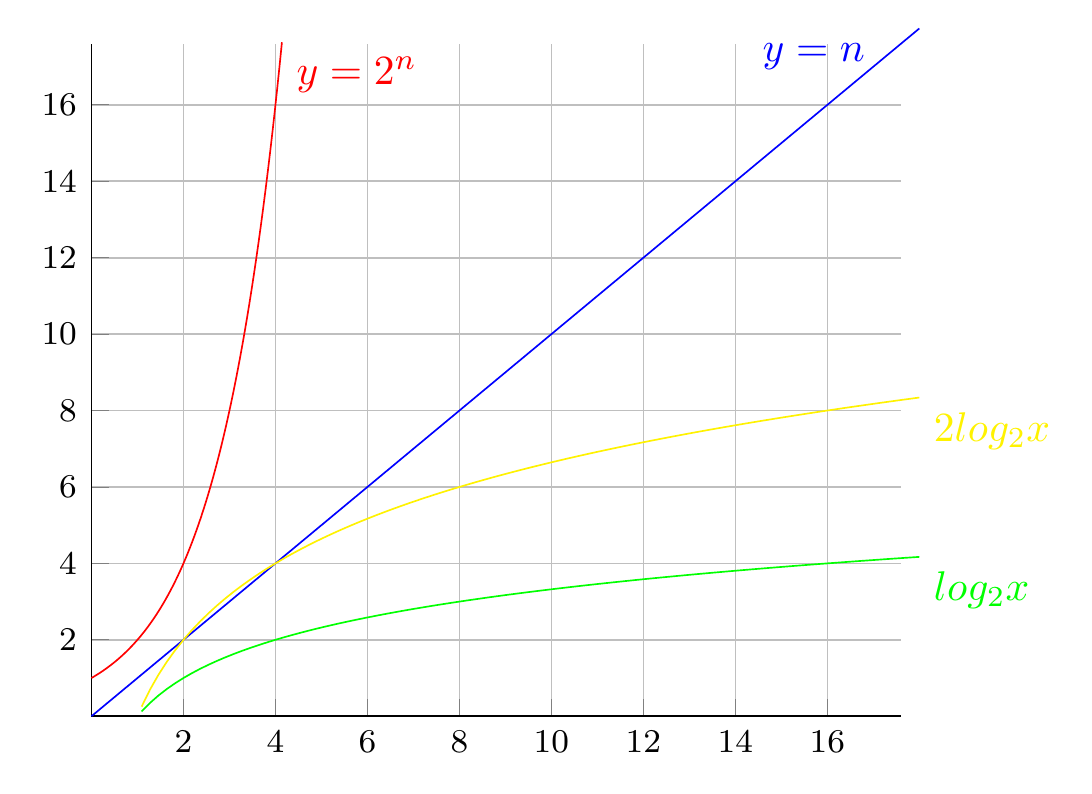
\begin{tikzpicture}[scale=1.5, transform shape]
\begin{axis}[grid=both,
      mark = none,
      xmin = 0, ymin = 0,
      xmax = 16,ymax = 16,
      axis lines*=middle,
      enlargelimits=upper,
      clip=false,
      xtick={0,2,...,16},
      ytick={0,2,...,16}]
\addplot[red, domain=0:5,restrict y to domain=0:18, samples=100]  {pow(2,x)} node[right,anchor=north west]{$y=2^n$};
\addplot[blue, domain=0:18,restrict y to domain=0:18, samples=100]  {x} node[anchor=north east,inner xsep=3ex] {$y=n$};
\addplot[green, domain=0:18,restrict y to domain=0:18, samples=100]  {ln(x)/ln(2)} node[right,anchor=north west]{$log_2x$};
\addplot[yellow, domain=0:18,restrict y to domain=0:18, samples=100]  {2*(ln(x)/ln(2))} node[right,anchor=north west]{$2log_2x$};
\end{axis}
\end{tikzpicture}
\end{center}
\section{Porównanie z innymi algorytmami sortującymi}
\section{Bibliografia}
\end{document}